% INFO6003 Final Report -- Version 3 (revised 15 October 2026).
% Revision: restructured around the author's actual five-stage, semi-automated workflow.
% Compile: pdflatex INFO6003_Final_Report_v3 (twice). Bibliography is embedded.
% Class: official Springer LNCS class llncs.cls v2.24 (2024/01/29), unmodified.
% Required file: figures/dbh_ecdf.pdf (generated by scripts/make_fig_dbh.py).
% Markers: [To be completed: ...] = evidence or values still to be supplied;
%          [VERIFY] = outside reference not checked against the original source.
% Status vocabulary used throughout: completed / in progress / planned / potential.
\documentclass[runningheads]{llncs}
\usepackage[T1]{fontenc}
\usepackage[utf8]{inputenc}
\usepackage{amsmath}
\usepackage{newtxtext}
\usepackage[varvw]{newtxmath}
\usepackage{graphicx}
\usepackage{booktabs,array}
\usepackage{tikz}
\usetikzlibrary{positioning,arrows.meta}
\usepackage{xurl}
\usepackage[hidelinks]{hyperref}
\usepackage{microtype}
\urlstyle{tt}

\newcommand{\todo}[1]{\textbf{[To be completed: #1]}}
\newcommand{\pend}{\textbf{[pending]}}
\newcommand{\verify}{\textbf{[VERIFY]}}
\newcommand{\figplaceholder}[2]{\fbox{\parbox[c][#1][c]{0.95\linewidth}{\centering\small\textbf{Figure placeholder.} #2}}}
\newcolumntype{L}[1]{>{\raggedright\arraybackslash}p{#1}}

\begin{document}
\title{Semi-Automated Individual-Tree Segmentation of Blue Mountains TLS Point Clouds: From Automated Extraction and Manual Refinement to Field Validation}
\titlerunning{Semi-Automated Individual-Tree Segmentation of Blue Mountains TLS Data}
\author{Tran Nguyen Gia Hung (Thomas) \todo{student ID}}
\authorrunning{T.\,N.\,G. Hung}
\institute{School of Computer, Data and Mathematical Sciences,\\Western Sydney University}
\maketitle

\begin{abstract}
Tree-level measurements from terrestrial laser scanning (TLS) require each point to be assigned to an individual tree, and automated segmentation remains unreliable where eucalypt crowns and branches overlap. This report documents a semi-automated workflow applied to TLS data from Blue Mountains forest plots: preparation of a large point cloud (PLY export, downsampling and extraction of regions of interest), automated terrain and tree extraction with RayCloudTools, manual refinement in CloudCompare, extraction of tree attributes, and comparison with field measurements. The first three stages have been carried out; manual refinement is the most time-consuming stage and is in progress. Attribute extraction and field validation are planned. I explain why manual refinement is needed, what it corrects and how it is controlled. A completed audit of the supplied plot inventory (1,507 site-linked records across 37 site identifiers) shows that field records cannot be matched to segmented trees without explicit rules: 88 records are logs or stumps, numbered diameter columns describe multiple stems rather than repeated censuses, 52 records lack a quadrant, and no tree coordinates are recorded. \todo{number of trees refined, refinement effort, and any attribute or validation results}. The contribution is a documented, reproducible semi-automated workflow and a curated individual-tree dataset, with conclusions limited to the evidence available.
\keywords{Terrestrial laser scanning \and Individual-tree segmentation \and Manual refinement \and Field inventory \and Reproducibility}
\end{abstract}

%======================================================================
\section{Introduction}\label{sec:intro}

\subsubsection{Motivation.}
Conventional forest inventories record species and stem diameter at breast height (DBH), whereas TLS captures the surfaces of stems, branches and crowns, enabling measurements such as branch architecture and woody volume that are impractical in the field~\cite{calders2020}. These tree-level products require each point to be assigned to one tree. Errors propagate: a merged crown inflates the attributes of one tree and removes those of another, and an omitted stem reduces completeness~\cite{calders2020,cherlet2026}. Segmentation remains the most challenging step to automate, and manual quality control is still needed, particularly in dense forests~\cite{cherlet2026,cushman2026}.

For the Blue Mountains monitoring network, the project team identified overlapping eucalypt crowns and complex branching as the main obstacles to automation, and noted that open forest needs less manual intervention than rainforest~\cite{meetingnotes}. The agreed approach is therefore semi-automated: automated extraction produces an initial segmentation, and manual review corrects it~\cite{meetingnotes,pipeline}. My project applies and documents this approach, with the aim of producing reliable individual-tree point clouds that can be measured and compared with field records.

\subsubsection{Research Questions and Objectives.}
The agreed minimum scope is a well-segmented plot, or a substantial portion of one, with biomass/allometric analysis and documentation; machine-learning automation, a second forest type and photogrammetry are stretch goals~\cite{meetingnotes}. Within that scope I address three questions:
\begin{itemize}
\item[\textbf{RQ1}] Which errors does automated Rayextract segmentation make in the selected area, and what does manual refinement change?
\item[\textbf{RQ2}] How much manual effort does refinement require, and which error types account for it?
\item[\textbf{RQ3}] How confidently can refined trees be associated with field records, and how closely do TLS-derived height and DBH agree with field measurements?
\end{itemize}
The objectives follow the workflow stages: (O1) prepare a tractable region of interest from the large TLS dataset; (O2) obtain an automated segmentation and document its errors; (O3) refine it manually into accepted individual-tree point clouds with a review log; (O4) extract tree attributes with scripted methods; and (O5) compare these attributes with field records under explicit matching rules. Biomass analysis remains part of the agreed scope \todo{confirm the final plot or region and any supervisor-approved change to the biomass objective}.

\subsubsection{Contribution and Status.}
I use existing tools and did not develop their algorithms~\cite{lowe2021,pipeline}. My contributions are: (C1, \emph{completed}) a scripted audit of the supplied plot inventory that fixes counting rules and quantifies the constraints on matching (Sect.~\ref{sec:res-inv}); (C2, \emph{in progress}) a curated set of individual-tree point clouds produced through documented manual refinement (Sects.~\ref{sec:manual} and~\ref{sec:res-proc}); and (C3, \emph{planned}) attribute extraction and field comparison (Sects.~\ref{sec:attr}--\ref{sec:valid}). Table~\ref{tab:stages} gives the status of every stage.

%======================================================================
\section{Related Work}\label{sec:related}

\subsubsection{From Point Clouds to Tree-Level Measurements.}
Calders et al.~\cite{calders2020} describe TLS processing as a chain of registration, tree extraction and modelling, e.g.\ quantitative structure models (QSMs). Most extraction methods grow detected stems bottom-up into crowns, and they usually need manual correction of omission and commission errors, more so in complex ecosystems where crowns interact. Downstream products inherit these errors: QSM quality depends on input-cloud quality, leaf-on data may require wood--leaf separation, and converting volume to biomass adds wood-density uncertainty~\cite{calders2020}.

\subsubsection{Automated Segmentation and Its Limits.}
Cherlet et al.~\cite{cherlet2026} benchmark five methods (Table~\ref{tab:methods}) on 2,983 manually segmented trees in four forest types, retaining ground, understory and unlabelled points so that methods face realistic clouds. The graph-based Rayextract achieved the highest plot-level F$_1$ on three of four plots and remained competitive on the fourth, but every method degraded in the dense tropical plot. Two findings explain why manual work persists. First, point-level accuracy fell with distance from the tree centre, which the authors attribute to interactions with neighbouring trees and small branches; errors therefore concentrate in the interlocking outer crown. Second, methods with similar scores can make different kinds of errors, so the authors expect qualitative assessment to remain part of semi-automated pipelines~\cite{cherlet2026}. Deep-learning models improved with fine-tuning, but were trained and tested on the same plots, which presupposes local labelled data.

\begin{table}[!tb]
\caption{Segmentation methods compared by Cherlet et al.~\cite{cherlet2026}. F$_1$ range: plot-level F$_1$ across their four test plots (their Table~2; deep-learning models fine-tuned on all plots).}\label{tab:methods}
\centering\footnotesize
\begin{tabular}{@{}L{1.45cm}L{4.0cm}L{3.6cm}c@{}}
\toprule
Method & Principle & Key dependency & F$_1$ range\\
\midrule
Rayextract & Shortest paths from terrain-mesh roots, agglomerated into trees & Terrain mesh; \texttt{height\_min}, \texttt{max\_diameter} & 0.480--0.919\\
Treeiso & Cut-pursuit graph clustering, then stem assignment & Ground and understory removed beforehand & 0.042--0.473\\
SSSC & Superpoint graph with wood probability; shortest paths to roots & Ground removal and height normalisation & 0.160--0.450\\
TreeLearn & Sparse-convolution network predicting offsets to tree base, then clustering & Labelled training data (in-domain fine-tuning) & 0.178--0.930\\
ForAINet & Network with offset and embedding branches, then clustering & Labelled training data (in-domain fine-tuning) & 0.247--0.905\\
\bottomrule
\end{tabular}
\end{table}

\subsubsection{Manual Segmentation as Reference and Bottleneck.}
Manual segmentation is regarded as the most accurate method, but it is labour-intensive, and operator bias remains in complex areas even after a second review pass~\cite{cherlet2026}. Cushman et al.~\cite{cushman2026} describe manual segmentation as a bottleneck in lidar studies of individual trees, note that processing time in dense forests can far exceed collection time, and stress that field measurements are themselves uncertain, so disagreement between TLS and inventory values cannot be attributed to the lidar side alone.

\subsubsection{Gap Addressed.}
None of the benchmark plots is a temperate sclerophyll eucalypt forest, and the benchmark leaves application-specific evaluation, such as inventory or biomass, to future work~\cite{cherlet2026}. My project addresses this gap locally by documenting what manual refinement changes in Blue Mountains data and by linking refined trees to field records under explicit, uncertainty-aware rules.

%======================================================================
\section{Data}\label{sec:data}

\subsection{TLS Dataset}\label{sec:tls}
The meeting notes describe 36 monitoring plots spanning dry sclerophyll forest (DSF), wet sclerophyll forest (WSF) and rainforest (RF), of which approximately 34 were scanned by Ghent University collaborators~\cite{meetingnotes}; the initial topic description refers to 35 plots~\cite{researchtopic} and the inventory contains 37 site identifiers, so the scanned population is not yet reconciled. I did not acquire the scans. The TLS dataset I work with covers a study area of more than one square kilometre and is exported to PLY, the input format used by RayCloudTools in the project pipeline~\cite{pipeline}. Its size makes processing at full resolution impractical, which motivates the preparation stage (Sect.~\ref{sec:prep}). \todo{scanner model, scan dates and positions, registration method and error, coordinate system, total extent and point count, and the location of the selected region of interest (Fig.~\ref{fig:manual}a)}.

\subsection{Field Reference Data}\label{sec:field}
Two inventory sources are relevant. The validation reference for Stage~5 is an Excel field inventory \todo{file name, custodian, version, fields available (e.g.\ tag, species, DBH, height), and how it relates to \texttt{TreeData.csv}}. Separately, I audited the supplied plot inventory \texttt{TreeData.csv}~\cite{treedata} (47 columns, 1,508 data rows), because its structure determines how any field record can be matched. One script applies these rules (Sect.~\ref{sec:repro}):
\begin{itemize}
\item \emph{Parsing.} Cells are read as trimmed strings; only \texttt{dbh1}--\texttt{dbh11} become numbers. Blanks stay missing and are never imputed; no non-blank diameter failed conversion. A final row without site, quadrant, species, tag or diameter is excluded and logged, leaving 1,507 site-linked records.
\item \emph{Counting.} Labels are counted as written; \texttt{log}, \texttt{stump} and \texttt{stump log} are reported separately. Status codes are lower-cased (changing one \texttt{L}). Sites are grouped by the leading letters DSF, WSF and RF.
\item \emph{Statistics and units.} Mean, sample SD ($n-1$), median, extremes and linearly interpolated quartiles; large values are kept and spellings are not repaired. Diameters stay in file units because the unit is undocumented \todo{DBH unit and protocol}.
\end{itemize}

\subsection{What Counts as a Tree?}\label{sec:target}
Inventory rows are not automatically segmentation targets. Besides logs and stumps, the labels include tree-fern genera (\textit{Dicksonia}, \textit{Cyathea}; 45 records) and, on my reading, climbers (\textit{Parsonsia}, \textit{Cissus}/\textit{Apocissus}; 11 records). Numbered diameter columns carry no dates, and notes such as ``two stems'' and ``multi stem'' accompany several populated slots in five of the six such records, so I interpret the slots as stems of one individual. No growth or multi-census comparison can therefore be computed. The file has no coordinate or height columns, so quadrant membership is the only spatial constraint for matching \todo{agreed target definition: growth forms, live/dead status, boundary trees, stem-versus-individual convention}.

%======================================================================
\section{Methodology and Implementation}\label{sec:method}

\subsection{Workflow Overview and Status}
Figure~\ref{fig:pipeline} and Table~\ref{tab:stages} summarise the five stages and their status. The stages are deliberately separated so that each output can be inspected and its effect on the final measurements traced: data preparation, automated processing, manual refinement, attribute extraction and validation.

\begin{figure}[!tb]
\centering
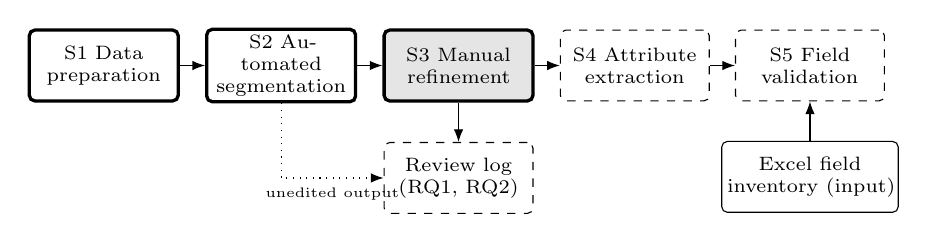
\begin{tikzpicture}[font=\scriptsize, node distance=3mm and 3.2mm,
  box/.style={draw, rounded corners=2pt, align=center, minimum height=9mm, text width=17.5mm, inner sep=2pt},
  done/.style={box, very thick},
  prog/.style={box, very thick, fill=black!10},
  plan/.style={box, dashed},
  arr/.style={-{Latex[length=1.6mm]}}]
\node[done] (s1) {S1 Data\\preparation};
\node[done, right=of s1] (s2) {S2 Automated\\segmentation};
\node[prog, right=of s2] (s3) {S3 Manual\\refinement};
\node[plan, right=of s3] (s4) {S4 Attribute\\extraction};
\node[plan, right=of s4] (s5) {S5 Field\\validation};
\node[plan, below=5mm of s3] (log) {Review log\\(RQ1, RQ2)};
\node[box, below=5mm of s5, text width=21mm] (inv) {Excel field\\inventory (input)};
\draw[arr] (s1)--(s2); \draw[arr] (s2)--(s3); \draw[arr] (s3)--(s4); \draw[arr] (s4)--(s5);
\draw[arr] (s3)--(log); \draw[arr] (inv)--(s5);
\draw[arr, dotted] (s2.south)|-node[pos=0.75,below,font=\tiny]{unedited output}(log.west);
\end{tikzpicture}
\caption{The five-stage semi-automated workflow. Thick border: carried out; shaded: in progress; dashed: planned. The unedited automated output is compared with the refined result to document errors (RQ1).}\label{fig:pipeline}
\end{figure}

\begin{table}[!tb]
\caption{Workflow stages, tools and status. ``Prior'' tools were developed by others and used without modification.}\label{tab:stages}
\centering\footnotesize
\begin{tabular}{@{}L{1.95cm}L{3.55cm}L{2.55cm}L{3.0cm}@{}}
\toprule
Stage & Main operations & Tools & Status\\
\midrule
S1 Preparation & PLY export, downsampling, ROI extraction & RiSCAN PRO / pipeline steps~\cite{pipeline} & Carried out \todo{settings}\\
S2 Automated & Terrain mesh, tree extraction, splitting into per-tree files & RayCloudTools (prior)~\cite{lowe2021} & Carried out \todo{run log}\\
S3 Manual & Error identification, branch reassignment, noise removal, acceptance check & CloudCompare (prior); propagation script~\cite{pipeline} & In progress \todo{trees accepted / total}\\
S4 Attributes & Height, DBH, other geometric attributes & Python scripts (mine) & Planned\\
S5 Validation & Matching to field records; agreement statistics & Python (mine) & Planned\\
Inventory audit & Counting rules, matching constraints & Python (mine) & Completed (Sect.~\ref{sec:res-inv})\\
\bottomrule
\end{tabular}
\end{table}

\subsection{Stage 1: Data Preparation}\label{sec:prep}
The large point cloud is exported to PLY, downsampled to reduce memory and processing time, and cropped to smaller regions of interest (ROIs) for detailed work~\cite{pipeline}. Both steps change the data that later stages see. Downsampling reduces point density on fine branches and thin stems, which may affect both segmentation and DBH fitting; a uniform point density is nevertheless recommended for consistent processing, for example through voxel-grid filtering~\cite{calders2020}. Cropping creates artificial boundaries that cut crowns and leave floating branches, which degrade segmentation near ROI edges~\cite{cherlet2026}. I therefore treat the downsampling resolution and ROI boundary as recorded parameters, and only trees whose stems lie well inside the ROI are candidates for validation \todo{downsampling method and resolution; ROI size, location and selection rationale; point counts before and after}.

\subsection{Stage 2: Automated Terrain and Tree Extraction}\label{sec:auto}
I process each ROI with RayCloudTools: \texttt{rayimport} converts the cloud to a ray cloud, \texttt{rayextract terrain} builds a terrain mesh, \texttt{rayextract trees} segments trees from that mesh, and \texttt{raysplit} and \texttt{treesplit} write per-tree outputs~\cite{pipeline}. Rayextract roots shortest paths in the terrain mesh, favours paths with consistent direction and from tall trees, and penalises strong lateral movement~\cite{cherlet2026}. This design suits upright stems but is a plausible source of error for long, lateral eucalypt branches that interlock with neighbouring crowns (a hypothesis that the review log will test).

The pipeline lists its example settings as ``parameters to check and optimise''~\cite{pipeline}. They differ from the benchmark's settings~\cite{cherlet2026} (its Sect.~3.1.1 and Table~A.1): the example terrain \texttt{gradient} is 2 (benchmark default 1); \texttt{height\_min} is 10, above the default (2) and every per-plot value (2.2--4.8), which may exclude smaller trees; and \texttt{max\_diameter} is 0.9, while twelve inventory records have \texttt{dbh1}~$>$~90 file units, which would exceed 0.9\,m if the unit is centimetres. I inspect the preliminary output visually before refinement \todo{the parameter values actually used and the reason for each}.

\subsection{Stage 3: Manual Refinement}\label{sec:manual}
\emph{Why it is necessary.} The automated output is a starting point, not a usable dataset. The literature and the project context identify four causes of error: overlapping crowns, in which branches of adjacent trees interlock and are assigned to the wrong stem; occlusion, which leaves gaps that break the connection between a branch and its stem; understory, climbers and other vegetation attached to stems; and noise from stray returns~\cite{calders2020,cherlet2026,cushman2026,meetingnotes}. Because errors concentrate in the outer crown~\cite{cherlet2026}, a tree can have a correct stem and a wrong crown, which would bias crown-based attributes and any biomass estimate.

\emph{What I correct.} Working tree by tree in CloudCompare, I (i) inspect each segment from several viewpoints; (ii) identify incorrectly assigned points; (iii) decide which branches belong to which tree by tracing each branch back to a stem; (iv) split merged trees and join fragments of one tree; (v) remove noise, unwanted vegetation and stray points; and (vi) check the result before accepting it. The project pipeline also produces a leftover cloud of unassigned points~\cite{pipeline}, which can be used to recover material the automated pass missed \todo{confirm whether the leftover cloud is used}. Deciding branch ownership where crowns interlock is the most difficult and time-consuming task, because the decision often depends on following thin, partly occluded branches through neighbouring crowns. Where ownership cannot be determined from the data, the case should be recorded as uncertain rather than resolved arbitrarily.

\emph{How quality is controlled.} The acceptance check is currently visual. To make it reproducible, I propose recording for each tree: a continuous stem from the ground; no branches attributed to a neighbour; no unexplained truncation of the crown; and removal of non-tree material \todo{confirm the criteria and whether they are recorded per tree}. Every point of the ROI cloud $P$ should end in exactly one accepted tree $T_k$, the leftover $L$, or an excluded set $X$:
\begin{equation}
|P| \;=\; \sum_{k=1}^{K}|T_k| \;+\; |L| \;+\; |X|, \qquad T_k\cap T_{k'}=\emptyset\ (k\neq k').
\end{equation}
A review log records tree ID, error type, edit, uncertainty and active time, and the unedited automated output is kept for comparison \todo{confirm that the unedited output was retained; number of trees refined and accepted; time spent}. Manual refinement has its own limits: it cannot recover unscanned structure, a single operator's decisions are subjective, and a reference derived by editing predictions may favour the automated baseline~\cite{cherlet2026}. A second reviewer checking a subset would reduce this dependence \todo{whether a second check is feasible}.

\subsection{Stage 4: Attribute Extraction (Planned)}\label{sec:attr}
Each accepted tree will be exported as a separate point-cloud file and processed with Python scripts. Tree height will be computed as the vertical distance from the terrain surface at the stem base to the highest point,
\begin{equation}
H_k = z_{\max}(T_k) - z_{\text{ground}}(x_k, y_k),
\end{equation}
using the terrain mesh from Stage~2. TLS can underestimate height because tree tops are sparsely sampled from the ground~\cite{calders2020,cushman2026}. DBH will be estimated from a thin horizontal slice of stem points at 1.3\,m above ground; slices of 3--10\,cm and circle-fitting algorithms are common~\cite{cushman2026}, but circle fits assume circular stems~\cite{calders2020}. Fit quality will be checked, and failed fits will remain in the denominator. Twenty-five inventory notes specify measurement above or below a fork, so the field and TLS diameters of those stems may not be comparable. Other attributes that a single-tree cloud supports, such as crown projected area from a convex hull~\cite{cushman2026}, may be added. I will not estimate tree age, because no validated age model or age data are available for these plots \todo{slice thickness, fitting method and quality rule}.

\subsection{Stage 5: Validation Against Field Records (Planned)}\label{sec:valid}
Matching uses the Excel field inventory (Sect.~\ref{sec:field}). Candidates are restricted to the confirmed site and quadrant, then compared on stem configuration and diameter; species is used only when identified independently, never inferred from the point cloud. I will solve a one-to-one assignment between refined trees $i$ and eligible records $j$, allowing either to remain unmatched, with diameter cost $C_{ij}=|\hat d_i-d_j|/s_d$, where $s_d$ is a justified scale \todo{scale, acceptance tolerance and multi-stem rule}. Matches will be reported as accepted, ambiguous or unmatched. Because selecting pairs by diameter and then validating diameter is circular, agreement statistics will be reported for independently identified pairs where possible, and otherwise labelled as conditional on the matching rule.

\subsection{Reproducibility, Environment and Data Availability}\label{sec:repro}
\emph{Environment.} The inventory audit was first run with Python~3.12.14, pandas~2.2.3 and NumPy~2.3.5, and re-executed with identical values under Python~3.13.16, pandas~3.0.5 and NumPy~2.5.3. The source CSV has SHA-256 \nolinkurl{fb308df06f978acd1fb48adf815c974a958b6312c72a45dd64d65722e1c44748}. \todo{RayCloudTools, CloudCompare and RiSCAN PRO versions; workstation specification}.

{\sloppy\emph{Repository.} The planned layout separates \texttt{scripts/} (audit, figure, attribute and matching code), \texttt{configs/} (Stage~1--2 settings), \texttt{logs/} (review, timing and association logs), \texttt{data/manifest.csv} (provenance and checksums; no restricted data) and \texttt{results/}. The audit and Fig.~\ref{fig:dbh} are regenerated by \texttt{python3 -I scripts/audit\_inventory.py data/TreeData.csv} and \texttt{scripts/make\_fig\_dbh.py} \todo{repository URL and committed layout}.\par}

\emph{Data availability.} Scans and inventories were supplied privately; public release requires custodian permission \todo{confirm}.

%======================================================================
\section{Experimental Evaluation}\label{sec:eval}
The evaluation is designed around the three questions, and each measure is tied to a recorded artefact.

\subsubsection{Automated versus Refined Segmentation (RQ1).}
Errors are classified from the review log as merges, splits, misassigned branches, omissions or non-tree material. Where the unedited automated output is retained, it will also be scored against the refined trees with the benchmark's procedure~\cite{cherlet2026}: one-to-one matching by point-set intersection-over-union, $\operatorname{IoU}(P_i,G_j)=|P_i\cap G_j|/|P_i\cup G_j|$, a detection threshold of IoU~$\geq$~0.5, and
\begin{equation}
\text{Precision}=\tfrac{TP}{TP+FP},\quad \text{Recall}=\tfrac{TP}{TP+FN},\quad F_1=\tfrac{2TP}{2TP+FP+FN},
\end{equation}
with point-level precision and recall reported for matched trees. Because the refined trees derive from the automated output, these scores measure how much refinement changed the result, not independent accuracy.

\subsubsection{Manual Effort (RQ2).}
Effort is reported as total and median active time per tree and the count of each edit type, from contemporaneous logs, excluding learning time and unattended computation. Effort will be compared between simple and overlapping-crown situations where the log allows.

\subsubsection{Agreement with Field Measurements (RQ3).}
For matched pairs with error $e_i=\hat d_i-d_i$, I report $\text{Bias}=\tfrac1n\sum e_i$, $\text{MAE}=\tfrac1n\sum|e_i|$ and $\text{RMSE}=\sqrt{\tfrac1n\sum e_i^2}$ for DBH, and for height if the Excel inventory contains heights, together with units, matching coverage and failed fits. The evaluation crop, eligible tree list and matching rules are fixed before any comparison is inspected \todo{crop, buffer and exclusion rules}.

%======================================================================
\section{Results}\label{sec:results}

\subsection{Processing Progress (Stages 1--3)}\label{sec:res-proc}
Stages~1 and~2 have been carried out on \todo{number and size of ROIs}, and manual refinement is in progress (Table~\ref{tab:pending}). Qualitatively, the preliminary Rayextract output required the corrections described in Sect.~\ref{sec:manual}: points assigned to the wrong tree, branches of overlapping crowns attributed to a neighbour, and noise, unwanted vegetation and stray points retained in tree segments. Separating overlapping branches has been the most time-consuming part of the work. These observations are not yet quantified; their frequency, distribution and cost will come from the review log (Fig.~\ref{fig:manual}b).

\begin{table}[!tb]
\caption{Quantities to be reported from the run logs, review log and validation. No values are reported yet.}\label{tab:pending}
\centering\footnotesize
\begin{tabular}{@{}lL{6.4cm}@{}}
\toprule
Stage & Quantity\\
\midrule
S1 & ROI area; downsampling resolution; points before/after \pend\\
S2 & Automated segments in ROI; segments discarded as non-tree \pend\\
S3 & Trees refined / accepted / uncertain; edits by type; active time per tree \pend\\
S3 vs S2 & Plot-level precision, recall, F$_1$ of unedited output against refined trees \pend\\
S4 & Height and DBH per tree; failed DBH fits \pend\\
S5 & Matched / ambiguous / unmatched records; DBH (and height) bias, MAE, RMSE \pend\\
\bottomrule
\end{tabular}
\end{table}

\begin{figure}[!tb]
\centering
\figplaceholder{1.8cm}{(a) Location of the ROI within the TLS dataset, with field quadrants. (b) The same trees before and after manual refinement, same view and scale, showing a reassigned overlapping branch and removed non-tree material \todo{produce from my CloudCompare sessions}.}
\caption{Region of interest (a) and an example of manual refinement (b).}\label{fig:manual}
\end{figure}

\subsection{Inventory Audit}\label{sec:res-inv}
Table~\ref{tab:coverage} summarises the 1,507 site-linked records in \texttt{TreeData.csv}. Of these, 88 carry deadwood-form labels (42 \texttt{log}, 34 \texttt{stump}, 12 \texttt{stump log}). The other 1,419 records use 63 identification strings, including seven \texttt{unknown Euc} and one \texttt{Unidentified}; they include probable spelling variants (e.g.\ \textit{Celestrus}, \textit{macrorhynca}) and overlapping names, which I have not merged. The most frequent labels are \textit{Corymbia gummifera} (274), \textit{Angophora costata} (86), \textit{Eucalyptus piperita} (86) and \textit{E.~sparsifolia} (84).

\begin{table}[!tb]
\caption{Site-linked inventory coverage by site prefix~\cite{treedata}. ``Other'' excludes only the three log/stump labels. Diameters in unconfirmed file units.}\label{tab:coverage}
\centering\footnotesize
\begin{tabular}{@{}lrrrrr@{}}
\toprule
Prefix & Site IDs & Records & Log/stump & Other & Median \texttt{dbh1}\\
\midrule
DSF & 26 & 1,096 & 55 & 1,041 & 17.00\\
WSF & 6 & 182 & 26 & 156 & 29.10\\
RF & 5 & 229 & 7 & 222 & 22.40\\
Total & 37 & 1,507 & 88 & 1,419 & 18.50\\
\bottomrule
\end{tabular}
\end{table}

\emph{Diameters.} The 1,506 numeric first-slot diameters (\texttt{dbh1}) have mean 24.14, SD 16.64, median 18.50, quartiles 13.20--29.58 and range 1.50--196.00 file units; excluding log/stump records ($n=1{,}419$), the median is 18.00. Pooling all eleven slots ($n=2{,}262$) lowers the mean to 19.72 because multi-stem records contribute smaller stems, not because of any temporal change. Of the records, 1,099 have one numeric diameter, 407 have two or more, and one stump has none; only 11 of the 1,419 non-log/stump first diameters fall below 10 file units (Fig.~\ref{fig:dbh}), consistent with, but not proof of, an inclusion threshold.

\begin{figure}[!tb]
\centering
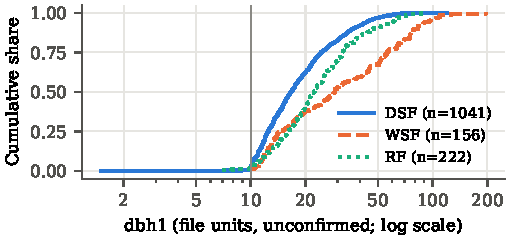
\includegraphics{figures/dbh_ecdf.pdf}
\caption{Cumulative distribution of first-slot diameter by site prefix, excluding log/stump labels (computed from~\cite{treedata}). The vertical line marks 10 file units.}\label{fig:dbh}
\end{figure}

\emph{Identity and status.} Quadrants are SW~379, SE~366, NE~358 and NW~352, with 52 missing (all records at \texttt{DSF\_M4A} and \texttt{WSF\_MH1B}). Tags include 115 \texttt{no\_tag} entries and six blanks; five identifiers recur across sites (ten records), and a note on both records of tag 1934 requests a field check. Tag alone is therefore not a valid key. In \texttt{live\_dead1}, records are 1,310 \texttt{l}, 196 \texttt{d} and one blank; the meaning of \texttt{l}/\texttt{d}, and of one \texttt{n} in later slots, is inferred from the column name only \todo{codebook}. Fifty-six notes mention ``outside'' or ``boundary''; these are review flags, not exclusions.

%======================================================================
\section{Discussion}\label{sec:discussion}

\subsubsection{What the Evidence Supports.}
Two conclusions are supported now. First, the automated output could not be used directly in my ROI: its errors (Sect.~\ref{sec:res-proc}) are consistent with the failure modes reported in the benchmark, which concentrate in the outer crown~\cite{cherlet2026}, so manual refinement is a necessary stage rather than an optional polish. This is a qualitative conclusion until the review log quantifies it. Second, the inventory audit shows that field matching must be site-qualified and ambiguity-aware, because tags recur, quadrants are missing and no coordinates exist (Sect.~\ref{sec:res-inv}).

\subsubsection{How Manual Refinement Contributes to Dataset Quality.}
Refinement changes what each file represents. Before it, a ``tree'' is whatever the path-based algorithm grew from one root, possibly including a neighbour's branches and attached vegetation; after it, each accepted file is intended to represent one individual that has passed a stated check, with uncertain cases flagged rather than hidden. This matters downstream: crown attributes, QSMs and biomass estimates depend on crown membership~\cite{calders2020}, and a learned segmenter trained on these files would inherit the conventions applied during refinement~\cite{cherlet2026}. The value of the refined dataset therefore depends on the consistency and documentation of refinement as much as on the number of trees processed, which is why the acceptance criteria and review log are part of the method.

\subsubsection{How Each Stage Can Affect the Final Measurements.}
The following are expectations to be tested, not findings. \emph{Downsampling} may thin fine branches and stems, weakening branch-ownership decisions and DBH fits for small trees. \emph{Automated segmentation} with a high \texttt{height\_min} may omit smaller trees (H1), and its lateral-path penalty may misassign interlocking eucalypt branches (H2). \emph{Manual refinement} should mainly change crown membership, so its effect on height and crown attributes is expected to exceed its effect on DBH, which depends on the lower stem (H3). \emph{Attribute extraction} adds its own error: occlusion of tree tops lowers TLS height~\cite{calders2020,cushman2026}, and non-circular or forked stems bias circle-fitted DBH. \emph{Field measurements} are also uncertain~\cite{cushman2026}. Disagreement between TLS and field values must therefore be interpreted with the matching evidence, not attributed to segmentation alone.

\subsubsection{Limitations.}
The main limitations are that attribute extraction and validation have not yet been carried out; that refinement effort and error frequencies are not yet quantified; that a single operator performs the refinement, which introduces subjectivity; that the refined trees are not independent of the automated output; that the study covers selected ROIs, not the full dataset; and that the relationship between the Excel inventory and \texttt{TreeData.csv} is not yet confirmed.

\subsubsection{Contribution and Potential Applications.}
The completed and ongoing work contributes a documented semi-automated workflow, an inventory audit with explicit matching constraints, and a growing set of refined individual-tree point clouds. If completed and validated, these could support: \emph{forest inventory and monitoring}, by providing tree-level height and DBH linked to plot records; \emph{structural analysis and biomass modelling}, since QSMs and woody-volume estimates require clean single-tree clouds~\cite{calders2020}; \emph{machine-learning research}, because the benchmark's deep-learning gains depended on local labelled training data~\cite{cherlet2026}, which refined trees could supply; and \emph{understanding of segmentation limits}, through an error log from a forest type absent from the benchmark. These are potential uses; none has been demonstrated in this project.

%======================================================================
\section{Conclusion and Future Work}\label{sec:conclusion}
This report presents the workflow as it has been carried out: a large TLS dataset is prepared through PLY export, downsampling and ROI extraction; RayCloudTools produces a preliminary segmentation; and manual refinement in CloudCompare corrects misassigned points, overlapping branches and non-tree material before each tree is accepted. Manual refinement has proved the most demanding stage, consistent with the literature on automated segmentation in complex forests. The completed inventory audit shows that field validation requires explicit target definitions and ambiguity-aware matching. Attribute extraction and field comparison are planned, and no accuracy claim is made yet \todo{update once Stage~3 is complete and Stages~4--5 have results}.

Next, I will complete and log the refinement, extract height and DBH with quality-checked scripts, match trees to the Excel inventory and report agreement with explicit denominators. A second forest type, a learned segmenter fine-tuned on the refined trees and QSM-based biomass remain future work.

\section*{Use of AI}
\todo{final declaration in the University's required wording. The subject outline requires that generative AI be used ``only as a support tool'' and ``declared in the submitted assessment in accordance with the University's Academic Integrity Policy''~\cite{info6003}. Draft: I used generative AI tools to summarise sources, re-run the inventory audit, and edit and format the text; I verified all numbers and citations myself.}

\begin{thebibliography}{9}
\bibitem{calders2020}
Calders, K., Adams, J., Armston, J., et al.: Terrestrial laser scanning in forest ecology: Expanding the horizon. Remote Sens. Environ. \textbf{251}, 112102 (2020). \href{https://doi.org/10.1016/j.rse.2020.112102}{doi:10.1016/j.rse.2020.112102}

\bibitem{cherlet2026}
Cherlet, W., Dayal, K., Chen, S., et al.: Benchmarking tree instance segmentation of terrestrial laser scanning point clouds. ISPRS J. Photogramm. Remote Sens. \textbf{231}, 230--247 (2026). \href{https://doi.org/10.1016/j.isprsjprs.2025.10.033}{doi:10.1016/j.isprsjprs.2025.10.033}

\bibitem{cushman2026}
Cushman, K.C., Kr\'al, K., Almeyda Zambrano, A.M., et al.: A primer on forest structure measurement with lidar for ecologists. Ecosphere \textbf{17}(8), e70730 (2026). \href{https://doi.org/10.1002/ecs2.70730}{doi:10.1002/ecs2.70730}

\bibitem{lowe2021}
Lowe, T.D., Stepanas, K.: RayCloudTools: A concise interface for analysis and manipulation of ray clouds. IEEE Access \textbf{9}, 79712--79724 (2021). \href{https://doi.org/10.1109/ACCESS.2021.3084954}{doi:10.1109/ACCESS.2021.3084954} \verify

\bibitem{meetingnotes}
Meeting notes, INFO6003 tree segmentation project (organiser B.~Choat). Unpublished (file dated 3 August 2026)

\bibitem{pipeline}
Steps processing pipeline (\nolinkurl{processing_pipeline.pdf}). Unpublished \todo{author, date}

\bibitem{treedata}
Blue Mountains plot inventory (\nolinkurl{TreeData.csv}). Unpublished dataset \todo{custodian, version}

\bibitem{researchtopic}
Research-topic description (\nolinkurl{Research-topic.txt}). Unpublished \todo{document to be re-checked}

\bibitem{info6003}
Western Sydney University: INFO6003 Postgraduate Research Project, Spring 2026 subject outline, Sects.~1.3 and 3.2.3 (2026)
\end{thebibliography}
\end{document}
